\chapter{Introduction}
\section{State of the art}

\section{Motivation and goals}

\section{Project planning and costs}
\subsection{Gantt diagram}
From the critical review to this final document there have been some changes to the planning. The most relevant is that we added a new work package to find a linear invariant metric to evaluate the stages proposed in this thesis. We also added a new work package for the oral presentation preparation.

Finally, the Gantt for this project is the following:
\begin{figure}[h!]
	\begin{center}
		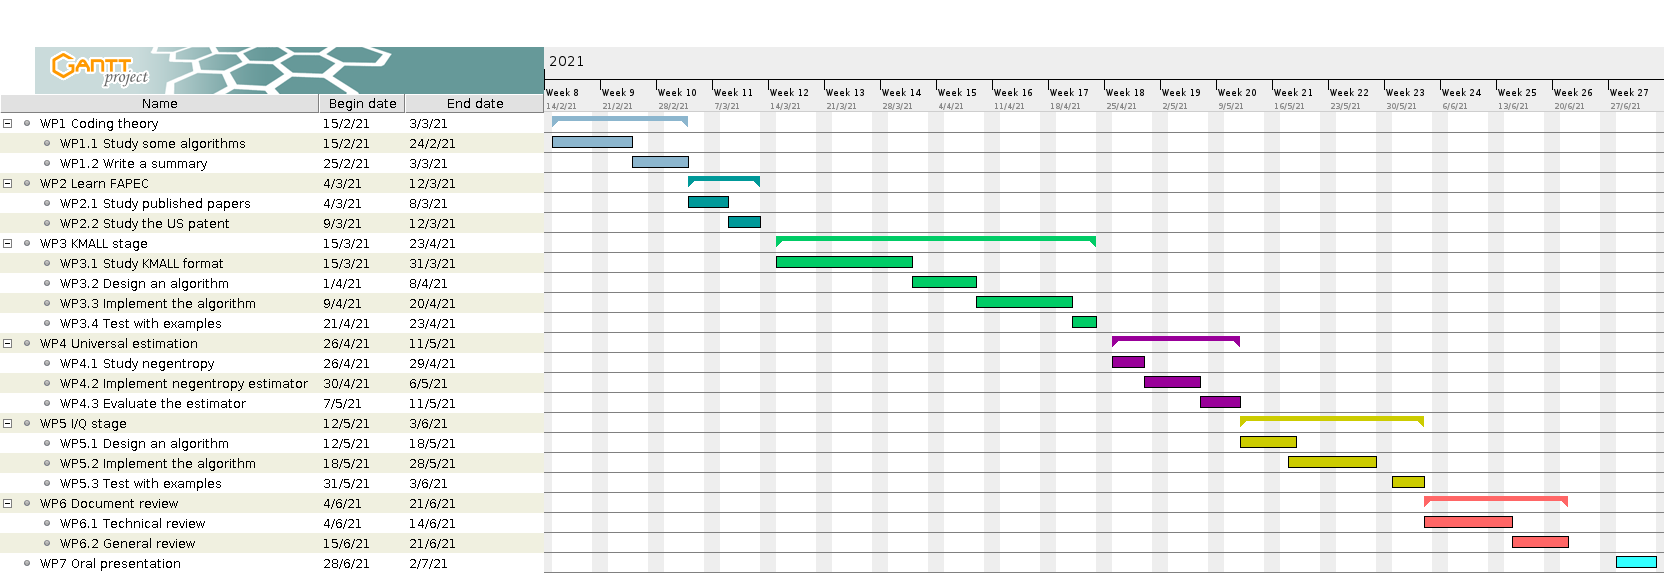
\includegraphics[scale=0.255]{images/gantt.png}
	\end{center}
	\caption{Final Gantt diagram.}
	\label{fig:gantt}
\end{figure}

\subsection{Budget and costs}
This thesis consists in the design, implementation and evaluation of two stages which will be included in a bigger framework, \acrshort{fapec}. In such situation, a financial study of only the stages is not possible, and studying the whole financial viability of \acrshort{fapec} is clearly out of the scope.

However, this thesis has been developed within a cooperation agreement between the Polytechnic University of Catalonia (UPC) and DAPCOM Data Services, with a cost of 3816€.

